\begin{frame}[c]
    \frametitle{使用集成滤光片阵列的高分辨率微型光谱仪的概念}
    \begin{columns}
        \begin{column}{.7\textwidth}
            \begin{itemize}
                \item Wang, S.-W.;  Xia, C.;  Chen, X.;  Lu, W.;  Li, M.;  Wang, H.;  Zheng, W.; Zhang, T., Concept of a \textcolor{purple}{high-resolution miniature spectrometer} using an \textcolor{red}{integrated filter array}. Optics letters 2007, 32 (6), 632-634.
                \item \textcolor{blue}{瓶颈:}滤光片阵列和 CCD 或检测器阵列之间可能会发生不对准,特别是对于具有非常小的元件尺寸和大集成度的滤光片阵列。边缘上的某些滤光片元件将与较少的 CCD 像素匹配,从而导致这些通道获得的信号较弱,并导致光谱中这些波长的信噪比相对较低。
                \item \textcolor{blue}{创新点:}同时具有极低的有效载荷、高分辨率和高可靠性等优点。
                \item 滤光片阵列具体结构(在下一篇文章中),CCD:SONY-ICX409AK
                \item \footnotesize{CCD:电荷耦合器件(Charge }Coupled Device)
            \end{itemize}
        \end{column}
        \begin{column}{.3\textwidth}
            \begin{figure}[H] %H为当前位置,!htb为忽略美学标准,htbp为浮动图形
                \centering %图片居中
                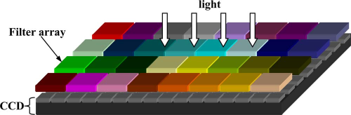
\includegraphics[width=1.\textwidth]{figures/Concept of a high-resolution miniature spectrometer using an integrated filter array_1.png} %插入图片,[]中设置图片大小,{}中是图片文件名
            \end{figure}
            \begin{figure}[H] %H为当前位置,!htb为忽略美学标准,htbp为浮动图形
                \centering %图片居中
                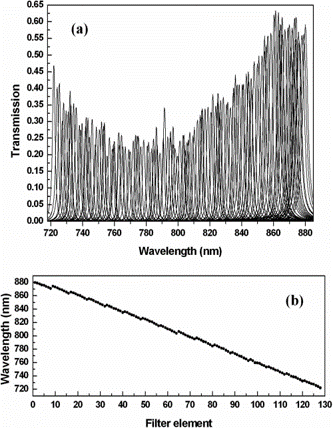
\includegraphics[width=1.\textwidth]{figures/Concept of a high-resolution miniature spectrometer using an integrated filter array_2.png} %插入图片,[]中设置图片大小,{}中是图片文件名
            \end{figure}
        \end{column}
    \end{columns}
\end{frame}

\begin{frame}[c]
    \frametitle{采用组合沉积技术快速制造128通道集成滤波器阵列}
    \begin{itemize}
        \item Wang, S.-W.;  Li, M.;  Xia, C.-S.;  Wang, H.-Q.;  Chen, X.-S.; Lu, W., \textcolor{purple}{128 channels of integrated filter array} rapidly fabricated by using the \textcolor{red}{combinatorial deposition technique}. Applied Physics B 2007, 88 (2), 281-284.
        \item \textcolor{blue}{创新点:}截至当时(2007)制作滤波器阵列最高效的组合方法。
        \item \textcolor{blue}{意义:}组合沉积技术(CDT)相对组合刻蚀技术(CET)简化了制备过程,减少了影响滤波器性能的因素。
    \end{itemize}
    \begin{figure}[H] %H为当前位置,!htb为忽略美学标准,htbp为浮动图形
        \centering %图片居中
        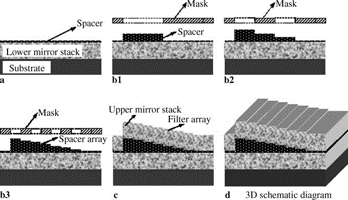
\includegraphics[width=1.\textwidth]{figures/128 channels of integrated filter array rapidly fabricated by using the combinatorial deposition technique_1.png} %插入图片,[]中设置图片大小,{}中是图片文件名
    \end{figure}
\end{frame}

\begin{frame}[c]
    \frametitle{128通道滤光片阵列}
    \begin{itemize}
        \item 全介质介质单腔滤光片
        \item 介质材料:H - $\mathrm{Nb_2O_5}$, L - $\mathrm{SiO_2}$, 中间介质 - $\mathrm{SiO_2}$
        \item 目标波长 $\lambda = 774 \text{nm}, \lambda/4 = 193.5 \text{nm}$
        \item 薄膜结构(共计29层):\begin{itemize}
                  \item 高反射膜堆 [L(193.5 nm)H(193.5 nm)LHLHLHLHLHLH]
                  \item (3.4 $\sim$ 5.1) $\times$ L(193.5 nm)
                  \item 高反射膜堆 [H(193.5 nm)L(193.5 nm)HLHLHLHLHLHL]
                  \item $\mathrm{Si}$ 基底
              \end{itemize}
    \end{itemize}
    \begin{columns}
        \begin{column}{.5\textwidth}
            \begin{figure}[H] %H为当前位置,!htb为忽略美学标准,htbp为浮动图形
                \centering %图片居中
                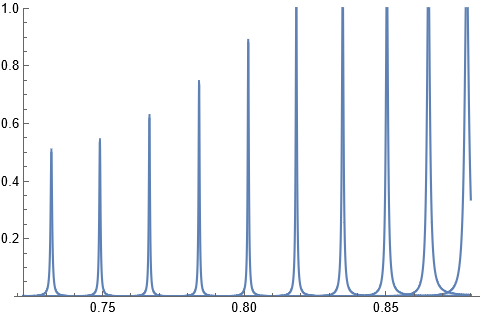
\includegraphics[width=1.\textwidth]{figures/128 channels of integrated filter array rapidly fabricated by using the combinatorial deposition technique_2.png} %插入图片,[]中设置图片大小,{}中是图片文件名
                \caption{10 通道} %最终文档中希望显示的图片标题
            \end{figure}
        \end{column}
        \begin{column}{.5\textwidth}
            \begin{figure}[H] %H为当前位置,!htb为忽略美学标准,htbp为浮动图形
                \centering %图片居中
                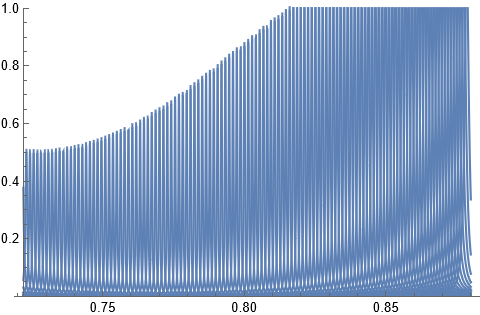
\includegraphics[width=1.\textwidth]{figures/128 channels of integrated filter array rapidly fabricated by using the combinatorial deposition technique_3.png} %插入图片,[]中设置图片大小,{}中是图片文件名
                \caption{128 通道} %最终文档中希望显示的图片标题
            \end{figure}
        \end{column}
    \end{columns}
\end{frame}

\begin{frame}[c]
    \frametitle{128通道滤光片阵列}
    \begin{itemize}
        \item 介质材料:H - $\mathrm{Nb_2O_5}$, L - $\mathrm{SiO_2}$, 中间介质 - $\mathrm{SiO_2}$
        \item 目标波长 $\lambda = 774 nm, \lambda/4 = 193.5 nm$
        \item 薄膜结构(共计29层):\\- 高反射膜堆(LHLHLHLHLHLHLH)\\- (3.4 $\sim$ 5.1) nm L\\- 高反射膜堆(HLHLHLHLHLHLHL)\\- $\mathrm{Si}$ 基底
    \end{itemize}
    \begin{figure}[H] %H为当前位置,!htb为忽略美学标准,htbp为浮动图形
        \centering %图片居中
        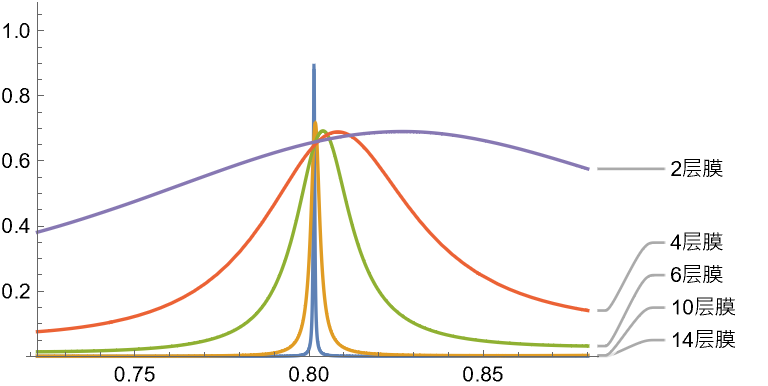
\includegraphics[width=.9\textwidth]{figures/128 channels of integrated filter array rapidly fabricated by using the combinatorial deposition technique_4.png} %插入图片,[]中设置图片大小,{}中是图片文件名
        \caption{高反射膜堆层数与透射率的关系} %最终文档中希望显示的图片标题
    \end{figure}
\end{frame}